\section{eo\-Continue$<$ EOT $>$ Class Template Reference}
\label{classeo_continue}\index{eoContinue@{eoContinue}}
Termination condition for the genetic algorithm Takes the population as input, returns true for continue, false for termination.  


{\tt \#include $<$eo\-Continue.h$>$}

Inheritance diagram for eo\-Continue$<$ EOT $>$::\begin{figure}[H]
\begin{center}
\leavevmode
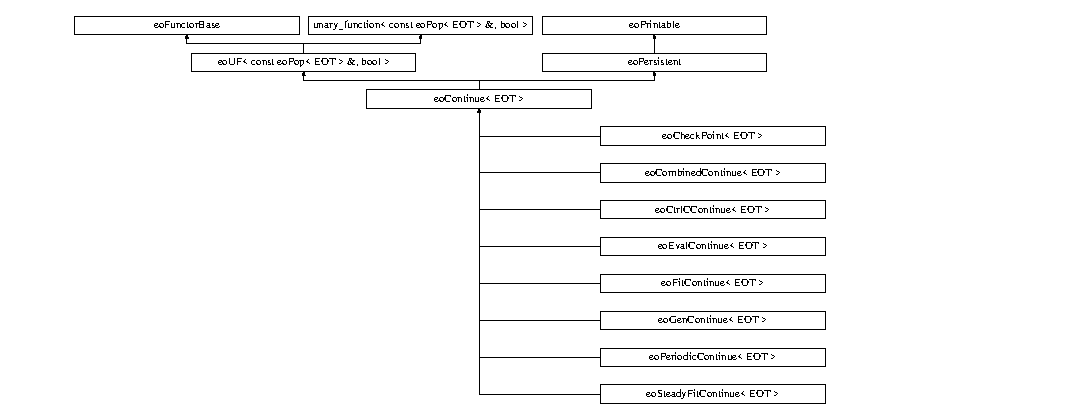
\includegraphics[height=5.2027cm]{classeo_continue}
\end{center}
\end{figure}
\subsection*{Public Member Functions}
\begin{CompactItemize}
\item 
virtual std::string {\bf class\-Name} (void) const \label{classeo_continue_a0}

\item 
void {\bf read\-From} (std::istream \&\_\-\_\-is)
\begin{CompactList}\small\item\em Read object. \item\end{CompactList}\item 
void {\bf print\-On} (std::ostream \&\_\-\_\-os) const 
\begin{CompactList}\small\item\em Write object. \item\end{CompactList}\end{CompactItemize}


\subsection{Detailed Description}
\subsubsection*{template$<$class EOT$>$ class eo\-Continue$<$ EOT $>$}

Termination condition for the genetic algorithm Takes the population as input, returns true for continue, false for termination. 



Definition at line 37 of file eo\-Continue.h.

\subsection{Member Function Documentation}
\index{eoContinue@{eo\-Continue}!readFrom@{readFrom}}
\index{readFrom@{readFrom}!eoContinue@{eo\-Continue}}
\subsubsection{\setlength{\rightskip}{0pt plus 5cm}template$<$class EOT$>$ void {\bf eo\-Continue}$<$ {\bf EOT} $>$::read\-From (std::istream \& {\em \_\-\_\-is})\hspace{0.3cm}{\tt  [inline, virtual]}}\label{classeo_continue_a1}


Read object. 

\begin{Desc}
\item[Parameters:]
\begin{description}
\item[{\em \_\-is}]A std::istream. \end{description}
\end{Desc}
\begin{Desc}
\item[Exceptions:]
\begin{description}
\item[{\em runtime\_\-std::exception}]If a valid object can't be read. \end{description}
\end{Desc}


Implements {\bf eo\-Persistent} {\rm (p.\,\pageref{classeo_persistent_a1})}.

Reimplemented in {\bf eo\-Gen\-Continue$<$ EOT $>$} {\rm (p.\,\pageref{classeo_gen_continue_a6})}.

Definition at line 42 of file eo\-Continue.h.\index{eoContinue@{eo\-Continue}!printOn@{printOn}}
\index{printOn@{printOn}!eoContinue@{eo\-Continue}}
\subsubsection{\setlength{\rightskip}{0pt plus 5cm}template$<$class EOT$>$ void {\bf eo\-Continue}$<$ {\bf EOT} $>$::print\-On (std::ostream \& {\em \_\-\_\-os}) const\hspace{0.3cm}{\tt  [inline, virtual]}}\label{classeo_continue_a2}


Write object. 

It's called print\-On since it prints the object on a stream. \begin{Desc}
\item[Parameters:]
\begin{description}
\item[{\em \_\-os}]A std::ostream. \end{description}
\end{Desc}


Implements {\bf eo\-Printable} {\rm (p.\,\pageref{classeo_printable_a1})}.

Reimplemented in {\bf eo\-Gen\-Continue$<$ EOT $>$} {\rm (p.\,\pageref{classeo_gen_continue_a7})}.

Definition at line 47 of file eo\-Continue.h.

The documentation for this class was generated from the following file:\begin{CompactItemize}
\item 
eo\-Continue.h\end{CompactItemize}
